\documentclass{article}
\usepackage{geometry}
\usepackage{float}
\usepackage[pdftex,colorlinks=true,linkcolor=red,citecolor=blue,urlcolor=black]{hyperref}
\usepackage{amsmath, amsthm, amssymb}
\usepackage{graphicx}
\usepackage{subfigure}
\usepackage{array}
\geometry{a4paper,scale=0.8}
\bibliographystyle{unsrt} %参考文献引用格式

\newcommand{\upcite}[1]{\textsuperscript{\cite{#1}}} %引用参考文献时,\upcite{1},能标在右上角,相当于是重定义一个语句。

\newcommand{\R}{\mathbb{R}}
\newcommand{\N}{\mathbb{N}}
\newcommand{\C}{\mathbb{C}}
\newcommand{\Z}{\mathbb{Z}}
\newcommand{\Q}{\mathbb{Q}}
\newcommand{\E}{\mathbb{E}}
\newcommand{\F}{\mathbb{F}}
\newcommand{\ip}[2]{\langle#1|#2 \rangle}
\newcommand{\hsip}[2]{\langle#1,#2 \rangle}
\newcommand{\braket}[1]{\langle#1 \rangle}
\newcommand{\sm}[1]{\left(\begin{smallmatrix} #1 \end{smallmatrix} \right)}

\DeclareMathOperator{\poly}{poly}
\DeclareMathOperator{\polylog}{polylog}
\DeclareMathOperator{\abs}{abs}
\DeclareMathOperator{\tr}{tr}
\DeclareMathOperator{\rank}{rank}
\DeclareMathOperator{\supp}{supp}
\DeclareMathOperator{\Var}{Var}
\DeclareMathOperator{\Inf}{Inf}
\DeclareMathOperator{\Cyc}{Cyc}
\DeclareMathOperator{\val}{val}
\DeclareMathOperator{\gap}{gap}


\newtheorem{theorem}{Theorem}
\newtheorem{lemma}[theorem]{Lemma}
\newtheorem{proposition}[theorem]{Proposition}
\newtheorem{corollary}[theorem]{Corollary}
\newtheorem{observation}[theorem]{Observation}
\newtheorem{definition}[theorem]{Definition}

\renewcommand{\theproposition}{\arabic{proposition}}

\title{Echo State Network for Image Classification}
\author{Fu Jiashen}

\begin{document}
\maketitle

\begin{abstract}
    This paper proposes a modified Echo State Network (ESN) model for image classification tasks. 
    The original ESN model is designed for sequence processing, which differs from the time-independent nature of image data. 
    To adapt the ESN to image classification, I propose two ways of modifications to the original ESN model.
    The simulation results on the MNIST dataset show that the modified ESN model can take on real-world image classification tasks,
    and is robust to adversal attacks.

    \textbf{Keywords:} Echo State Network, Image Classification, Adversal Attack

\end{abstract}

\section{Introduction}

Echo State Network\upcite{ESN} (ESN) is a type of Recurrent Neural Network (RNN) 
that is designed for sequence processing. The design of the reservoir makes it possible for the ESN
to capture the temporal dependencies in the input data. The echo state property of the reservoir layer 
makes it possible for the ESN to have a desired attractor property, i.e., for the input data under the 
same class, the hidden states of the reservoir layer will converge to a similar state. Moreover, as shown in Fig. \ref{fig:sequence_distance}, for different sequences, the hidden states of the reservoir layer
are attracted to different areas in the state space. This makes it possible for the ESN model 
to classify the sequences correctly. The ESN model has been successfully applied to a variety of sequence classification tasks, 
such as audio classification\upcite{ESN_audio}, 
human eye movement classification\upcite{ESN_human_eye}, etc.

\begin{figure}[htbp]
    \centering
    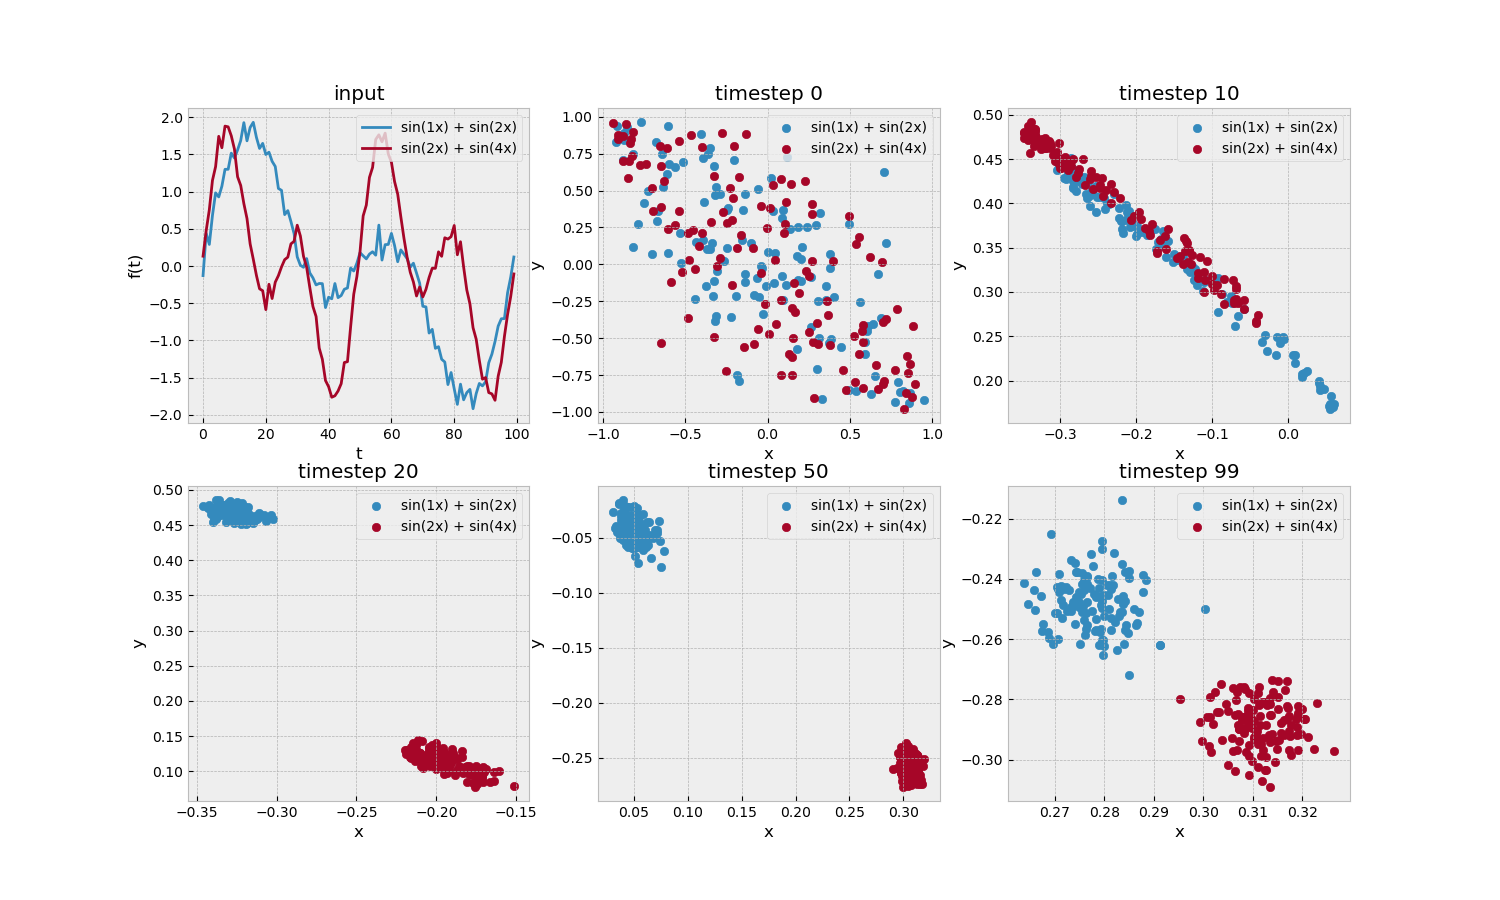
\includegraphics[width=0.9\textwidth]{assets/sequence_distance.png}
    \caption{Simulation results for sequence classification. 
    The upper-left figure shows the input data, while the other
    figures show the 2-dimensional hidden states of the reservoir layer at 
    different time steps.}
    \label{fig:sequence_distance}
\end{figure}


Herbert Jaeger\upcite{ESN} shows that the hidden states of the reservoir have a desirable continuity: 
For all left-infinite input sequences $\bar u^{-\infty}$, for all $\epsilon > 0$, there exists a $\delta > 0$ 
and a $h > 0$ such that $d(x, x') < \epsilon$ for all left-infinite input sequences $\bar u'^{-\infty}$ which 
satisfy $d(\bar u^{-\infty}(k), \bar u'^{-\infty}(k)) < \delta$ for all $-h < k < 0$, where $x$ and $x'$ are 
the final hidden states of the reservoir layer. For small perturbations in the input data, 
the hidden states of the reservoir layer will converge to a similar state.
This property makes the ESN model robust to small perturbations 
in the input data. Thus makes it less vulnerable to adversal attacks\upcite{Adversarial}.

However, the ESN model is not suitable for image classification tasks, as the input data is not time-dependent.
This paper proposes a modified ESN model for image classification tasks.


\section{Related Work}

\subsection{Echo State Network}

Echo State Network is a special class of reservoir computing. The original ESN model\upcite{ESN} is composed of three layers:
input layer, reservoir layer and output layer. The reservoir layer is a recurrent neural network with a fixed weight matrix. 
If we denote the input data at time $t$ as $u(t)$, the hidden states of the reservoir layer at time $t$ as $x(t)$, and the 
output of the model at time $t$ as $y(t)$, then the ESN model can be described by the following equations:

\begin{equation}
    x(t) = f(W_{in}u(t) + W_{res}x(t-1) + W_{back}y(t-1))
\end{equation}

\begin{equation}
    y(t) = f^{out}(W_{output}(x(t), u(t), y(t-1)))
\end{equation}

where $f$ is the activation function of the reservoir layer, $f^{out}$ is the activation function of the output layer,
$W_{in}$ is the weight matrix of the input layer, $W_{res}$ is the weight matrix of the reservoir layer, $W_{back}$ is the weight matrix
of the feedback loop, and $W_{output}$ is the weight matrix of the output layer. Only $W_{output}$ is trainable.


The most important property of the ESN model is the echo state property of the reservoir layer.

\begin{definition}
    (Echo State Property\upcite{ESN}) Assume standard compactness conditions. Assume that the
    network has no output feedback connections. Then, the network has echo
    states, i.e., for a given left-infinite input sequence $\bar u^{-\infty}(i), \quad i=...,n-1,n$, and hidden 
    states $x(i) = T(x(i-1), u(i))$ and $x'(i) = T(x'(i-1), u(i))$ , we have $x'(n) = x(n)$, where $T$ is the
    transition function of the reservoir layer.
\end{definition}

In other words, the hidden states of the reservoir layer will converge to the same state for a given input sequence, no matter what the initial state is.

\begin{figure}[htbp]
    \centering
    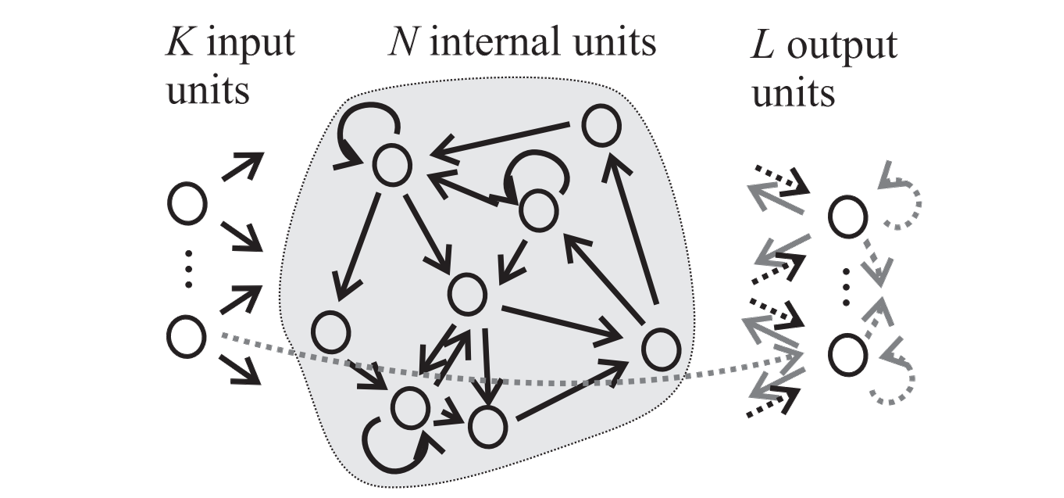
\includegraphics[width=0.8\textwidth]{assets/esn.png}
    \caption{The original Echo State Network model. Credit to Herbert Jaeger\upcite{ESN}}
    \label{fig:esn_original}
\end{figure}

Herbert Jaeger\upcite{ESN} proposed a simple method to guarantee the echo state property of the reservoir layer:

\begin{proposition}
    Assume a sigmoid network with unit output functions $f = tanh$. 
    Let the weight matrix W satisfy $\sigma_{max} = \Lambda < 1$, 
    where $\sigma_{max}$ is the
    largest singular value of W. Then the network has an echo state.
\end{proposition}

Thus, we can simply choose the weight matrix $W_{res}$ randomly from a normal distribution, and scale it to a fixed spectral radius less than 1,
then the echo state property of the reservoir layer is guaranteed.


\subsection{Adversal Attack}

Adversal robustness\upcite{Adversarial} is a notorious problem in deep learning. It is shown that deep learning models are vulnerable to small perturbations
in the input data. And the adversal noise is the strongest perturbation that can miss lead the model to make wrong predictions.
Formally, given a deep learning model $f$, an input data $x$ and its original label $y$, 
the adversal attack problem is to find a small perturbation $\epsilon$ such that $f(x + \epsilon) \neq y$.

The most common adversal attack method is the Projected Gradient Descent (PGD)\upcite{PGD} method. The PGD method is an iterative method, which
iteratively updates the input data so that the loss function is amplified. The update rule is given by:

\begin{equation}
	x_{t+1} = \prod_{x+S}(x_t+\alpha sign (\nabla_x L(x_t,y;\theta))
\end{equation}

where $x$ is the input data, $S$ is the set of allowed perturbations, $\alpha$ is the step size, 
$L$ is the loss function, and $\theta$ is the parameters of the model. This method is
considered the strongest attack method based on the first-order gradient information.
And it is the adversal attack method used in this paper.


\section{The Model}

The original Echo State Network \upcite{ESN} (ESN) is designed for sequence processing, which differs from the time-independent nature of 
image data. To adapt the ESN to image classification, I propose two ways of modifications to the original ESN model, 
denoted as Type I and Type II respectively.

\begin{figure}[htbp]
    \centering
    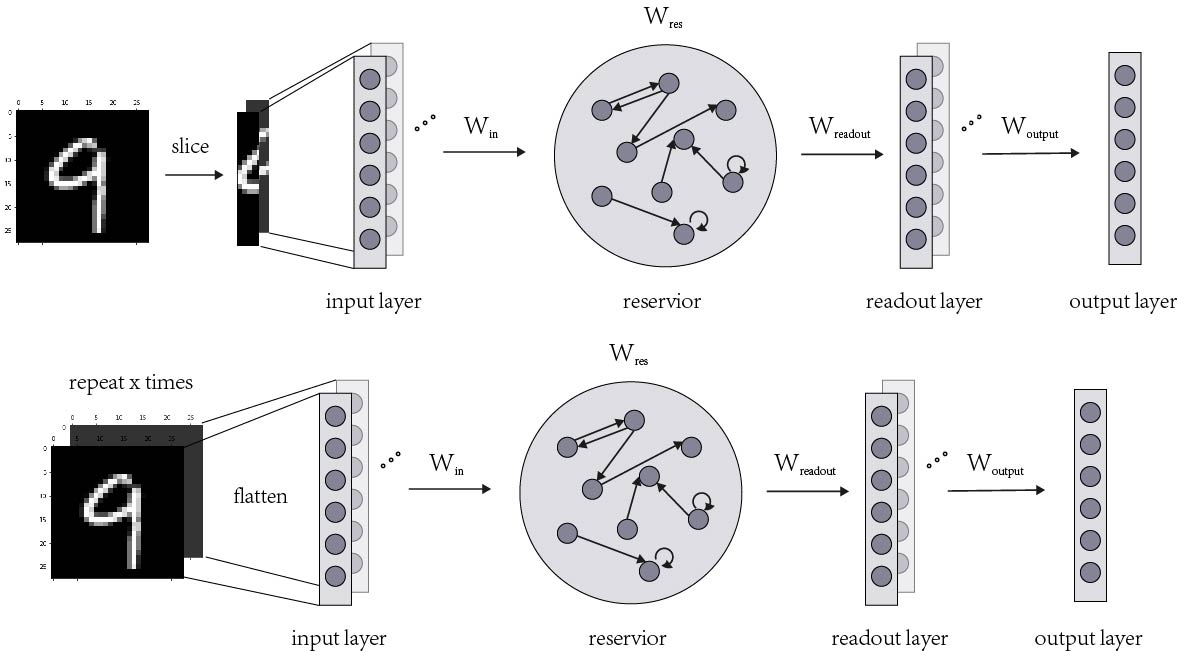
\includegraphics[width=0.8\textwidth]{assets/esn.jpg}
    \caption{Illustration for the modified Echo State Network Type I(above) and Type II(below).}
    \label{fig:esn}
\end{figure}

As shown in Fig. \ref{fig:esn}, the modified ESN is composed of four layers: input layer ($u(t)$), reservoir layer ($x(t)$), 
readout layer ($h(t)$) and output layer ($y(t)$).
The reservoir layer and readout layer are the same as the original ESN, which are calculated by the following equations:

\begin{equation}
    x(t) = tanh(W_{in}u(t) + W_{res}x(t-1))
\end{equation}

\begin{equation}
    h(t) = tanh(W_{readout}x(t))
\end{equation}

The output layer is calculated based on the concatention of the readout layer at every time step, 
so that the features extracted by the reservoir layer at different time steps can be fully utilized:

\begin{equation}
    y(t) = softmax(W_{output}(\bigcup_{t}h(t)))
\end{equation}

where the softmax function is defined as:

\begin{equation}
    softmax(x) = \frac{e^{x}}{\sum_{i}e^{x_i}}
\end{equation}

One can see the output of softmax function as the probability of different classification labels.
The final classification result is determined by the label with the highest probability.

Type I and Type II (see Fig. \ref{fig:esn}) differ in the way of constructing the input layer.
The Echo State Network is good at capturing the temporal dependencies in the input data, so
it is a natural choice to use the input data in a sequential way. Type I splits 
the image column-wise, and feeds the pixels of each column into the network sequentially.
Thus the spatial dependency of image data is turned into a temporal dependency. In comparison,
Type II simply repeats the image data for a fixed number of times, 
and feeds the repeated data into the network. 

Among the parameters, $W_{in}$ is chosen randomly from a uniform distribution,
and $W_{res}$ is chosen randomly from a normal distribution, then scaled to a fixed spectral radius.
$W_{readout}$ and $W_{output}$ are trainable.

\section{Results} 
\label{sec:results}

Source code available at \url{https://github.com/Jason-Fu-git/EchoStateNetworkForImageClassification}.

The experiment is conducted on the MNIST dataset, which contains 60,000 training images 
and 10,000 testing images. The images have 28x28 pixels, and can be classified into 10 classes.

The hyperparameters of the model are set as follows: 1. the size of the input layer is 28 for Type I, and 
28x28 for Type II; 2. the size of the reservoir layer is 500 for both types; 3. the size of 
the readout and output layer is 10 for both types; 4. the sparsity of $W_{in}$ and $W_{res}$ is 0.1
for both types.

The model is trained for 10 epochs, using Adam\upcite{Adam} optimizer with a learning rate of 0.01, 0.001, 0.0001 for
different stages and a weight decay of 3e-4.

\begin{table}[htbp]
    \centering
    \caption{Classification accuracy for different spectral radius values}
    \begin{tabular}{c|ccccc}
        \hline
        Spectral radius & 0.1   & 0.5   & 0.9   & 1.0   & 1.5   \\ \hline
        Type I          & 0.9434 & 0.9477 & 0.9567 & 0.9470 & 0.8248 \\
        Type II         & 0.9336 & 0.9312 & 0.9291 & 0.9257 & 0.9130 \\ \hline
    \end{tabular}
    \label{tab:spectral_radius_clean}
\end{table}


Table \ref{tab:spectral_radius_clean} shows the classification accuracy for different spectral radius values
and different types of the model. The best classification accuracy is 0.9567, demonstrating the effectiveness
of the modified ESN model for image classification. For Type I, when the spectral radius is less than 1, the
choice of spectral radius has little impact on the classification accuracy. However, when the spectral radius
is greater than 1, the accuracy drops significantly. This is because when the reservoir losses its echo state property,
the model is no longer capable of capturing the temporal dependencies in the input data. For Type II, the classification
accuracy does not change much with the spectral radius, which is consistent with the fact that the input data is not
time-dependent.


\begin{table}[htbp]
    \centering
    \caption{Classification accuracy for different spectral radius values under PGD\upcite{PGD} attack}
    \begin{tabular}{c|ccccc}
        \hline
        Spectral radius & 0.1   & 0.5   & 0.9   & 1.0   & 1.5   \\ \hline
        Type I          & 0.9126 & 0.9195 & 0.9287 & 0.9153 & 0.7868 \\
        Type II         & 0.8385 & 0.8263 & 0.7825 & 0.7674 & 0.8499 \\ \hline
    \end{tabular}
    \label{tab:spectral_radius_adversal}
\end{table}


Table \ref{tab:spectral_radius_adversal} shows the classification accuracy for different spectral radius values
and different types of the model under PGD\upcite{PGD} attack with epsilon of 4/255. The result of Type I does not
differ much from the clean data, which indicates that processing the image data in a sequential way is robust to 
adversal noises. However, the result of Type II drops significantly, which suggests that simply repeating the image data
is not robust to adversal noises. This result indicates that Type I is more robust and learns better than Type II, thus 
more suitable for undertaking image classification tasks.


\begin{table}[htbp]
    \centering
    \caption{Type II model's classification accuracy for different numbers of iteration }
    \begin{tabular}{c|ccccc}
        \hline
        Iteration number& 1   & 5   & 10   & 20             \\ \hline
        Clean data      & 0.6458 & 0.9194 & 0.9253 & 0.9332 \\ 
        Under PGD\upcite{PGD} attack& 0.5929 & 0.8209 & 0.8078 & 0.8040 \\ \hline
    \end{tabular}
    \label{tab:num_iters}
\end{table}

Table \ref{tab:num_iters} shows the classification accuracy of Type II model for different numbers of iteration.
The result shows that when the number of iteration is greater than 5, the reservoir layer exhibits the echo state property,
and the classification accuracy remains at a high level.


\section{Discussion}

The results in Section \ref{sec:results} shows that the modified ESN model can compete with the state-of-the-art deep learning models
in image classification tasks. Model Type I takes less parameters, performs better and is more robust than Model Type II. 
Its effectiveness can be credited to the echo state property of the reservoir layer, which gives the model
an "attractor property", i.e., for different samples under the same class, the hidden states of the reservoir will converge to a similar state.
This property is illustrated in Fig. \ref{fig:cosine_similarity}, which shows that, when the samples are under the same class, 
the hidden states of the reservoir layer exhibit a high cosine similarity. However, when the samples are under different classes, the hidden states 
differs significantly.


\begin{figure}[htbp]
    \centering
    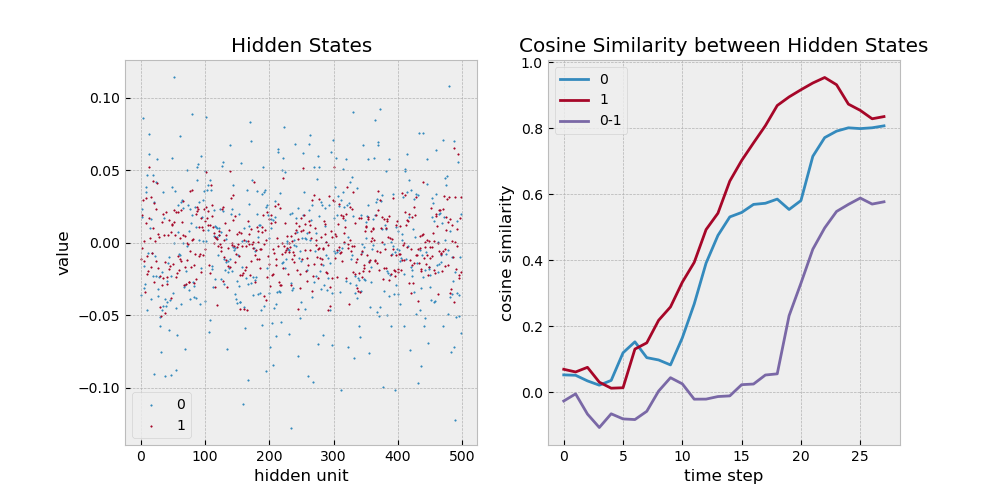
\includegraphics[width=0.8\textwidth]{assets/cosine_similarity.png}
    \caption{Difference between the hidden states}
    \label{fig:cosine_similarity}
\end{figure}


However, this "attractor property" can also be a problem. It is possible that when the input data under different classes are close to each other, 
the hidden states of the reservoir layer will converge to a similar state, which will lead to misclassification. 
This is illustrated in Fig. \ref{fig:attractor_problem}. The input data are 2-D points randomly sampled from two Gaussian distributions centered 
at (2, 4) and (4, 2) respectively. The hidden states are very close to each other, which makes it hard for the model to classify the data correctly.

\begin{figure}[htbp]
    \centering
    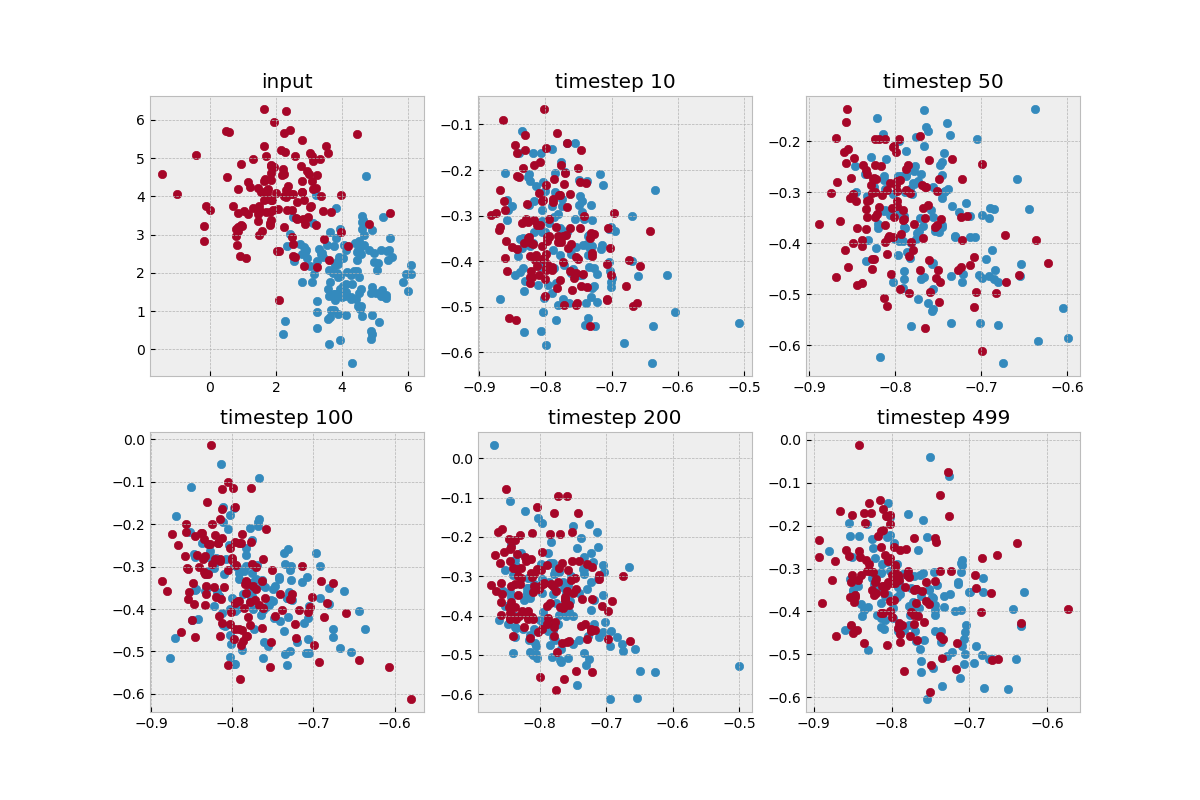
\includegraphics[width=0.8\textwidth]{assets/attractor_problem.png}
    \caption{Input data (upper left) and hidden states of the reservoir layer at different time steps}
    \label{fig:attractor_problem}
\end{figure}

This problem can be attributed to the fact the reservoir layer is not trainable. It does not know which "direction" the hidden state should be drawn to.
Different data under different classes may be drawn close to each other. To alleviate the problem, one can make the reservoir layer trainable, so that 
the reservoir layer can learn the diffence between the different classes. This shows the potential of the modified ESN model for further improvement.

\clearpage

\section*{Acknowledgment}

This paper is the final project of the course "Research Methods in Psychology and AI" at Tsinghua University.
I would like to thank the instructor, Prof. Mi, for her guidance and support. I would also like to 
thank TA Feng and TA Zhang for their efforts.

\bibliography{cite}

\end{document}